\setlength{\parindent}{1em}
\renewcommand{\thesection}{\Alph{section}}
\renewcommand{\thesubsection}{\thesection.\arabic{subsection}}

\noindent\begin{minipage}[t]{0.48\textwidth}
{\large\bfseries Appendix Contents}\par\medskip\small
\begin{tabular}{@{}p{0.82\linewidth}r@{}}
\textbf{\ref{app:proof}\quad Proofs and Analysis} & \textbf{\pageref{app:proof}}\\
\quad\ref{app:proofprop}\quad Proof of Proposition~\ref{prop:lift} & \pageref{app:proofprop}\\
\quad\ref{app:cliff}\quad Why a slip allowance is a cliff & \pageref{app:cliff}\\
\textbf{\ref{app:sim}\quad Simulation Details} & \textbf{\pageref{app:sim}}\\
\quad\ref{app:model}\quad Model and parameters & \pageref{app:model}\\
\quad\ref{app:devlog}\quad Development decisions & \pageref{app:devlog}\\
\quad\ref{app:val}\quad Rig validation & \pageref{app:val}\\
\textbf{\ref{app:ctrl}\quad Controller, Shield and Training} & \textbf{\pageref{app:ctrl}}\\
\quad\ref{app:code}\quad Probe, bound and shield code & \pageref{app:code}\\
\quad\ref{app:train}\quad Training details & \pageref{app:train}\\
\textbf{\ref{app:main}\quad Additional Main Results} & \textbf{\pageref{app:main}}\\
\textbf{\ref{app:ext}\quad Extended Study Details} & \textbf{\pageref{app:ext}}\\
\textbf{\ref{app:protocol}\quad Protocol, Deviations, Reproducibility} & \textbf{\pageref{app:protocol}}\\
\end{tabular}
\end{minipage}\hfill
\begin{minipage}[t]{0.48\textwidth}
{\large\bfseries List of Appendix Figures and Tables}\par\medskip\small
\begin{tabular}{@{}p{0.82\linewidth}r@{}}
Fig.~\ref{fig:cliffapp}\quad Certified grip vs.\ assumed drop & \pageref{fig:cliffapp}\\
Fig.~\ref{fig:validation}\quad Rig validation & \pageref{fig:validation}\\
Fig.~\ref{fig:training}\quad Training curves & \pageref{fig:training}\\
Fig.~\ref{fig:gallery}\quad All failures of the worst seed & \pageref{fig:gallery}\\
Table~\ref{tab:params}\quad Simulation parameters & \pageref{tab:params}\\
Table~\ref{tab:hyper}\quad Training hyperparameters & \pageref{tab:hyper}\\
Table~\ref{tab:perr}\quad Test set, all methods and $r$ & \pageref{tab:perr}\\
Table~\ref{tab:perseed}\quad Per-seed results & \pageref{tab:perseed}\\
Table~\ref{tab:confirm}\quad Confirmation set & \pageref{tab:confirm}\\
Table~\ref{tab:rmax}\quad Mismatched $r_{\max}$ & \pageref{tab:rmax}\\
Table~\ref{tab:perobj}\quad Per-object results & \pageref{tab:perobj}\\
Fig.~\ref{fig:ctrltime}\quad Controlled study: lift time & \pageref{fig:ctrltime}\\
Table~\ref{tab:changes}\quad Controlled changes & \pageref{tab:changes}\\
Table~\ref{tab:controlled}\quad Controlled study, absolute & \pageref{tab:controlled}\\

Table~\ref{tab:compute}\quad Compute & \pageref{tab:compute}\\
\end{tabular}
\end{minipage}
\clearpage

\section{Proofs and Analysis}\label{app:proof}
\subsection{Proof of Proposition~\ref{prop:lift}}\label{app:proofprop}
\textbf{Setting.} The rod (mass $m$) is held between two pads, each pressing with normal force $F$. Let $x(t)\ge0$ be the
downward displacement of the rod relative to the fingers and $v=\dot x$. The palm, and with it the fingers, moves up with
acceleration $a(t)$. In the palm frame the rod feels gravity plus the inertial force, a downward demand of $m(g+a)$ per
unit time, and a friction force from the two pads opposing relative motion. With Coulomb friction and a static-to-kinetic
drop:
\begin{itemize}
\item while stuck ($v=0$), the friction force can take any value up to $2\mu_sF$, so the rod stays stuck while
$m(g+a)\le2\mu_sF$;
\item while sliding down ($v>0$), the friction force is $2\mu_kF$ upward, so $m\dot v=m(g+a)-2\mu_kF$.
\end{itemize}
\textbf{Step 1 (what the probe certifies).} The probe observed the rod stuck at grip $\Fs$ with the palm at rest ($a=0$)
for 0.3\,s. Hence $mg\le2\mu_s\Fs$, i.e.\ $\Fs\ge F_b:=mg/(2\mu_s)$. For any grip $F$ the static capacity per unit mass is
$2\mu_sF/m=gF/F_b\ge gF/\Fs$.

\textbf{Step 2 (no slip before $t_0$).} For $t<t_0$, $g+a(t)\le gF/\Fs\le2\mu_sF/m$, so the stick condition holds and
$x(t)=v(t)=0$.

\textbf{Step 3 (relative acceleration after $t_0$).} With $r=\mu_s/\mu_k\le r_{\max}$, the kinetic capacity per unit mass is
$2\mu_kF/m=gF/(rF_b)\ge gF/(r_{\max}\Fs)$. Whenever the rod slides, $\dot v=g+a-2\mu_kF/m\le\bar a$. Whenever it is stuck,
$\dot v=0$, and $v=0\le\bar v$.

\textbf{Step 4 (comparison).} Let $\bar v$ solve $\dot{\bar v}=\bar a$ with $\bar v$ clipped at zero, from $\bar v(t_0)=0$.
Suppose $v(t)>\bar v(t)$ for some $t$, and let $t_1=\sup\{s<t:\ v(s)\le\bar v(s)\}$. On $(t_1,t]$ we have $v>\bar v\ge0$, so the
rod slides and $\dot v\le\bar a\le\dot{\bar v}$ wherever $\bar v>0$; where $\bar v=0$ is clipped, $\bar a\le0$ and again
$\dot v\le\bar a\le0$. Integrating from $t_1$, where $v(t_1)\le\bar v(t_1)$ by continuity, gives $v(t)\le\bar v(t)$, a
contradiction. Hence $v\le\bar v$ for all $t\ge t_0$, and $x(t)=\int_{t_0}^t v\le\int_{t_0}^t\bar v=\bar s(t)$.\hfill$\square$

\textbf{What the proof does not cover.} (i) Elastic compliance: the rod can move relative to the fingers without slipping
by deforming the contact; we measured 0.1--0.5\,mm and cover it with the 1.5\,mm margin. (ii) Rate dependence and
pre-sliding friction~\cite{canudas1995}: the proof assumes a static level that holds up to breakaway and a single kinetic
level after it. (iii) Loss of grasp: once the rod's end passes the pads, there is no friction at all; this only happens for
bounds of many centimetres, which the shield never certifies. (iv) The grip ramp: our grip ramps down to $F$ over 0.3\,s
from a higher grip, so using $F$ throughout the rest phase is conservative.

\subsection{Why a slip allowance is a cliff}\label{app:cliff}
\textbf{Scale invariance.} Proposition~\ref{prop:lift} depends on the grip only through $\rho=F/\Fs$: the onset condition is
$g+a(t)>g\rho$ and $\bar a=g+a-g\rho/r_{\max}$. The certified grip is therefore $F^\star=\Fs\,\rho^\star(T,r_{\max},s_{\lim})$
and its ratio to the no-onset grip $F_{\rm model}=\Fs(g+a_{pk})/g$ is a function of $T$, $r_{\max}$ and $s_{\lim}$ only. This
is why the ratio was identical for all 40 test objects.

\textbf{The cliff.} Write $\rho=(1-\varepsilon)(g+a_{pk})/g$ for a grip a fraction $\varepsilon$ below the no-onset grip.
Slip may begin a little before the acceleration peak, at the first $t_0$ with $a(t_0)>a_{pk}-\varepsilon(g+a_{pk})$. From
then on the bound integrates
\begin{equation}
\bar a(t)=g+a(t)-\frac{(1-\varepsilon)(g+a_{pk})}{r_{\max}}
=\underbrace{\big(a(t)-a_{pk}\big)+\varepsilon(g+a_{pk})}_{\text{as without a drop}}+\underbrace{(1-\varepsilon)(g+a_{pk})\Big(1-\frac1{r_{\max}}\Big)}_{\text{kinetic deficit}} .
\end{equation}
Without a drop ($r_{\max}=1$) only the first term acts; it is positive only near the peak and integrates to a small slip
that grows smoothly with $\varepsilon$. With a drop, the second term is a constant of order $(g+a_{pk})(1-1/r_{\max})$: for
$T=0.37$\,s and $r_{\max}=1.2$ it is about $2.3$\,m/s$^2$, larger than the first term's whole positive range for small
$\varepsilon$. It keeps $\bar v$ growing until the minimum-jerk profile decelerates enough to cancel it, roughly a third of
the lift later, so even an infinitesimal $\varepsilon$ certifies centimetres of slip. The certified grip therefore sits at
$\varepsilon=0$ unless the allowance $s_{\lim}$ is larger than this jump. Figure~\ref{fig:cliffapp} shows the result for
three allowances and three lift durations.

\begin{figure}[h]\centering
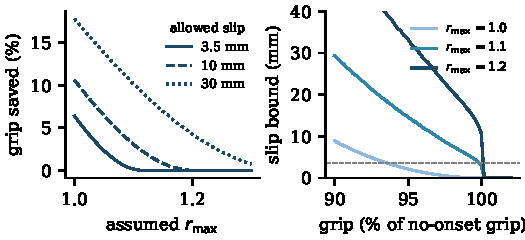
\includegraphics[width=0.62\textwidth]{fig_cliff.pdf}
\caption{\textbf{The cliff.} Left: grip saved by allowing 3.5, 10 or 30\,mm of slip at $T=0.37$\,s, as a function of the assumed
drop $r_{\max}$. Right: Proposition~\ref{prop:lift}'s bound as a function of grip for three values of $r_{\max}$; with any
drop, the bound jumps from zero to centimetres as soon as slip can begin.}\label{fig:cliffapp}
\end{figure}

\begin{table}[h]\centering\small
\caption{\textbf{Grip saved by a slip allowance} (\% of the no-onset grip), computed from Proposition~\ref{prop:lift}; the values
are the same for every object.}\label{tab:allow}
\begin{tabular}{@{}ccrrrrrrr@{}}\toprule
$T$ (s) & allowance (mm) & $r_{\max}=1.0$ & $r_{\max}=1.02$ & $r_{\max}=1.05$ & $r_{\max}=1.1$ & $r_{\max}=1.15$ & $r_{\max}=1.2$ & $r_{\max}=1.3$\\\midrule
0.37 & 3.5 & 6.38 & 4.59 & 2.30 & 0.15 & 0.00 & 0.00 & 0.00\\
0.37 & 10 & 10.60 & 8.85 & 6.45 & 3.07 & 0.83 & 0.00 & 0.00\\
0.37 & 30 & 17.81 & 16.18 & 13.83 & 10.15 & 6.94 & 4.22 & 0.74\\
0.50 & 3.5 & 4.04 & 2.27 & 0.43 & 0.00 & 0.00 & 0.00 & 0.00\\
0.50 & 10 & 6.72 & 4.93 & 2.61 & 0.23 & 0.00 & 0.00 & 0.00\\
0.50 & 30 & 11.28 & 9.54 & 7.10 & 3.61 & 1.12 & 0.02 & 0.00\\
1.00 & 3.5 & 1.18 & -0.00 & -0.00 & -0.00 & -0.00 & -0.00 & -0.00\\
1.00 & 10 & 1.96 & 0.36 & -0.00 & -0.00 & -0.00 & -0.00 & -0.00\\
1.00 & 30 & 3.29 & 1.53 & 0.02 & -0.00 & -0.00 & -0.00 & -0.00\\
\bottomrule\end{tabular}
\end{table}

\clearpage
\section{Simulation Details}\label{app:sim}
\subsection{Model and parameters}\label{app:model}
Listing~\ref{lst:xml} is the complete MuJoCo model; \texttt{\{m\}} and \texttt{\{mu\}} are filled per object. The palm body
is massive (1000\,kg), gravity-compensated and driven kinematically: before and after every physics step its slide joint's
position and velocity are overwritten with the planned trajectory, so the pads move with the planned acceleration
regardless of contact forces. Table~\ref{tab:params} lists every parameter.

\begin{codebox}{MuJoCo model (Listing \thelstlisting)}
\lstinputlisting[style=xml,label=lst:xml]{code_xml.xml}
\end{codebox}

\begin{codebox}{Stick--slip emulation: one physics step}
\lstinputlisting[style=py]{code_mj1.py}
\end{codebox}

\begin{table}[h]\centering\small
\caption{\textbf{Simulation and task parameters.}}\label{tab:params}
\begin{tabular}{@{}llll@{}}\toprule
Parameter & Value & Parameter & Value\\\midrule
time step & 1\,ms (implicit-fast) & friction cone & elliptic, impedance ratio 10\\
no-slip iterations & 20 & pad geometry & spheres, radius 6\,mm, condim 4\\
contact solref / solimp & 0.003, 1 / 0.95, 0.99, 0.0005 & torsional / rolling friction & 0.005 / 0.0001\\
rod & box 2$\times$2$\times$16\,cm on vertical slide & finger joints & slide, damping 300, force control\\
object mass $m$ & $U[0.05,0.2]$\,kg & static friction $\mu_s$ & $U[0.4,0.8]$\\
kinetic switch & $|v_{\rm rel}|>2$\,cm/s; back below 2\,mm/s & ratio $r$ (test) & 1.0, 1.1, 1.2, 1.3\\
lift height $H$ & 10\,cm & lift profile & minimum jerk\\
grip ramp + settle & 0.3\,s + 0.3\,s & hold after lift & 0.3\,s\\
slip tolerance $S_{\rm tol}$ & 5\,mm & sensing margin & 1.5\,mm\\
slip-monitor noise & 0.5\,mm (Gaussian) & weight estimate & $m\cdot U[0.9,1.1]$\\
probe start & $\hat mg/(2\cdot0.3)$ & probe step & $\times0.9$ per 0.4\,s\\
probe motion threshold & 2.5\,mm & probe re-clamp & $2.5\times$ moving grip in 20\,ms\\
maximum grip & 30\,N & model lift time $T_0$ & 1\,s\\
shield $r_{\max}$ & 1.2 & lift time range & 0.25--2\,s\\\bottomrule
\end{tabular}\end{table}

\subsection{Development decisions}\label{app:devlog}
The rig went through several versions before the protocol was frozen. We list every change that affected behaviour, in
order, because each one is a modelling choice a reader may want to revisit. None was made after a policy was trained.
\begin{enumerate}[leftmargin=1.5em]
\item \textbf{Driven palm.} A mocap (teleported) palm has no velocity, so contact friction never dragged the rod upward.
We replaced it with a slide joint whose position and velocity are imposed.
\item \textbf{Gravity compensation.} The palm sagged under gravity within each step and the rod crept; we made the palm heavy
(1000\,kg) and gravity-compensated.
\item \textbf{Reactive probe.} With $r>1$, holding a probe grip that turned out too low let the rod slide away. The probe now
watches the slip and re-clamps at once.
\item \textbf{Re-clamp level.} Snapping to the maximum grip and then ramping down produced long, large ramps; the probe now
snaps to 2.5 times the grip that moved, and the lift's grip ramp lasts 0.3\,s. The bound's rest phase was lengthened to
match (0.6\,s).
\item \textbf{Switching thresholds.} Slow elastic creep at the original 5\,mm/s threshold switched rods to kinetic friction
although they were not slipping; we raised the thresholds to 2\,cm/s and 2\,mm/s.
\item \textbf{Axial slide.} A free rod rocked about the grasp axis after slip (about 0.24\,rad/s) and crept afterwards, so the
model controller dropped objects with a zero bound. We constrained the rod to a vertical slide. After this change the model
controller held 40 of 40 development objects at $r\in[1,1.2]$.
\end{enumerate}

\subsection{Rig validation}\label{app:val}
\textbf{V1} measures the grip at which a rod first moves with the palm still, by bisection over grips, for 20 development
objects at $r=1$, against $mg/(2\mu_s)$. \textbf{V2} does the same during lifts of duration 0.25--1\,s, against the
quasi-static $m(g+a_{pk})/(2\mu_s)$. \textbf{V3} runs 120 complete episodes with a probe, $r\sim U[1,1.2]$, a random
duration $T\sim U[0.25,1]$\,s and a random grip between 0.6 and 1.4 times the quasi-static need, and compares the measured
slip with the bound at $r_{\max}=1.2$. \textbf{V4} measures creep in well-held lifts at four grip margins.
Figure~\ref{fig:validation} shows the results. The bound is loose wherever it is non-zero, often by one to two orders of
magnitude (panel b): with $\Fs$ above the true breakaway grip and the quasi-static model conservative for fast lifts, a rod
that the bound allows to slip usually does not slip at all. This looseness is one reason the shield ends up forbidding slip
altogether; Section~\ref{sec:extended} measures it directly.

\begin{figure}[h]\centering
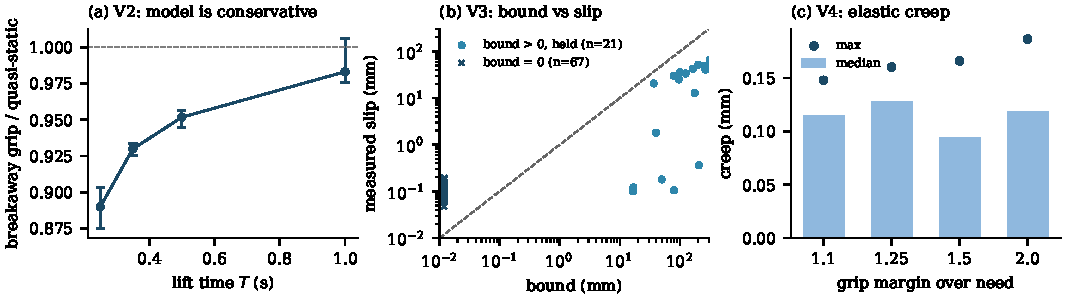
\includegraphics[width=\textwidth]{fig_validation.pdf}
\caption{\textbf{Rig validation.} (a) Breakaway grip during a lift relative to the quasi-static prediction (mean and range over
8 objects). (b) Bound against measured slip in 120 random lifts (log axes; zero bounds drawn at the left edge; 32 dropped
rods, all with bounds above 0.5\,m, omitted). (c) Elastic creep in well-held lifts.}\label{fig:validation}
\end{figure}

\clearpage
\section{Controller, Shield and Training}\label{app:ctrl}
\subsection{Probe, bound and shield code}\label{app:code}
The listings below are copied verbatim from \texttt{lift\_env.py} by a script, so they match the code that produced every
result.

\begin{codebox}{Probe: reactive search for the breakaway grip}
\lstinputlisting[style=py]{code_probe.py}
\end{codebox}

\begin{codebox}{Proposition~\ref{prop:lift}: the slip bound over the whole commanded profile}
\lstinputlisting[style=py]{code_lift_bound.py}
\end{codebox}

\begin{codebox}{Shield projections: grip axis and time axis}
\lstinputlisting[style=py]{code_shield_grip.py}
\vspace{2pt}
\lstinputlisting[style=py]{code_shield_time.py}
\end{codebox}

\begin{codebox}{One episode, all methods}
\lstinputlisting[style=py]{code_model_grip.py}
\lstinputlisting[style=py]{code_features.py}
\lstinputlisting[style=py]{code_run_episode.py}
\lstinputlisting[style=py]{code_score.py}
\end{codebox}

\subsection{Training details}\label{app:train}
Each iteration samples 6 training objects ($r\sim U[1,1.2]$) and their episode seeds, draws 6 Gaussian perturbations
$\epsilon_i$ of the $2\times6$ weight matrix, and evaluates the policy at $w\pm\sigma\epsilon_i$ on all 6 objects, plus the
current policy. Rewards are rank-transformed to $[-0.5,0.5]$ and the gradient estimate
$\sum_i(\mathrm{rank}^+_i-\mathrm{rank}^-_i)\epsilon_i/(6\sigma)$ is followed with Adam~\cite{salimans2017,kingma2015}.
Table~\ref{tab:hyper} lists the settings, which are those of our earlier residual papers~\cite{aidoo2026b,aidoo2026c}, unchanged.

\begin{table}[h]\centering\small
\caption{\textbf{Training hyperparameters} (identical for B2 and B5).}\label{tab:hyper}
\begin{tabular}{@{}ll@{\hspace{2em}}ll@{}}\toprule
antithetic pairs & 6 & objects per iteration & 6\\
perturbation scale $\sigma$ & 0.1 & Adam step & 0.06 ($\beta=0.9,0.999$)\\
iterations & 20 & episodes per run & 1{,}560\\
initial weights & 0 (model controller) & seeds & 0--4\\
duration scale & $T=T_0e^{1.0a_T}$ & grip scale & $F=F_{\rm model}(T)e^{0.25a_F}$\\
failure reward & $-10$ & success reward & $-T/T_0-\lambda F/(10mg)$, $\lambda=1$\\\bottomrule
\end{tabular}\end{table}

\begin{codebox}{Training loop (\texttt{train\_es.py})}
\lstinputlisting[style=py]{code_train.py}
\end{codebox}

\begin{figure}[h]\centering
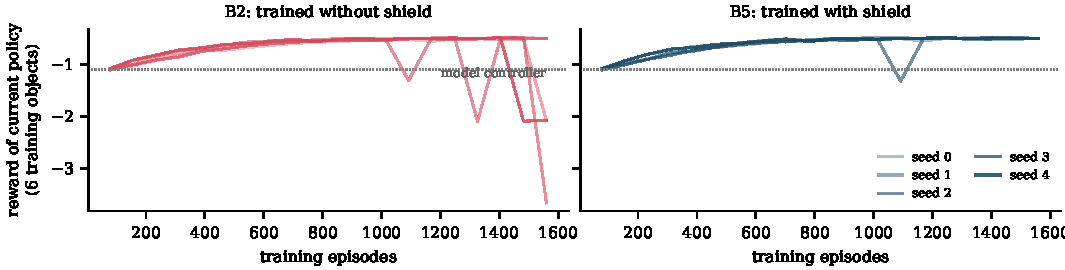
\includegraphics[width=\textwidth]{fig_training.pdf}
\caption{\textbf{Training curves.} Reward of the current (unperturbed) policy on each iteration's 6 training objects. Both
methods improve on the model controller (dotted) within about 600 episodes. The unshielded runs dip whenever an iteration's
batch contains a lift that slips: three of the five B2 runs ended on such a batch. The shielded runs never fail and converge
to the same reward, about $-0.50$.}\label{fig:training}
\end{figure}

\clearpage
\section{Additional Main Results}\label{app:main}
Tables~\ref{tab:perr}--\ref{tab:perobj} give the complete test-set and confirmation results behind Section~\ref{sec:results}.
Figure~\ref{fig:gallery} shows every failure of the worst B2 seed.

\begin{table*}[!htbp]\centering\footnotesize
\caption{\textbf{Test set, every method at every $r$} ($r_{\max}=1.2$). Failure counts with Wilson 95\% intervals (\%);
$\Delta T$ and $\Delta F/mg$ against B0 with hierarchical bootstrap 95\% intervals (seeds, then objects); ``obj.\ worse'' counts
objects that failed at least once under the method but never under B0, with the Holm-corrected exact McNemar $p$ (B0S and B4t are
outside the pre-registered Holm families and show the raw $p$). All lift-time and grip differences have Holm-corrected Wilcoxon
$p<10^{-10}$.}\label{tab:perr}
\setlength{\tabcolsep}{4pt}
\begin{tabular}{@{}lrrllrrr@{}}\toprule
Method & failures & Wilson CI (\%) & $\Delta T$ (s) & $\Delta F/mg$ & obj.\ worse & $p$ & max slip (mm)\\\midrule
\multicolumn{8}{@{}l}{\textit{$r=1.0$}}\\
B0 & 0/40 & [0.0, 8.8] & --{\scriptsize} & --{\scriptsize} & -- & -- & 0.49\\
B0S & 0/40 & [0.0, 8.8] & +0.000{\scriptsize} & +0.000{\scriptsize} & 0 & 1 & 0.49\\
B2 & 3/200 & [0.5, 4.3] & -0.628{\scriptsize [-0.629, -0.627]} & +0.267{\scriptsize [+0.237, +0.304]} & 2 & 1 & 8.59\\
B4g & 0/200 & [0.0, 1.9] & -0.628{\scriptsize [-0.629, -0.627]} & +0.350{\scriptsize [+0.328, +0.372]} & 0 & 1 & 0.12\\
B4t & 0/200 & [0.0, 1.9] & -0.581{\scriptsize [-0.597, -0.566]} & +0.267{\scriptsize [+0.237, +0.303]} & 0 & 1 & 0.14\\
B5 & 0/200 & [0.0, 1.9] & -0.630{\scriptsize [-0.630, -0.629]} & +0.352{\scriptsize [+0.330, +0.374]} & 0 & 1 & 0.11\\
\multicolumn{8}{@{}l}{\textit{$r=1.1$}}\\
B0 & 0/40 & [0.0, 8.8] & --{\scriptsize} & --{\scriptsize} & -- & -- & 0.49\\
B0S & 0/40 & [0.0, 8.8] & +0.000{\scriptsize} & +0.000{\scriptsize} & 0 & 1 & 0.49\\
B2 & 25/200 & [8.6, 17.8] & -0.628{\scriptsize [-0.629, -0.627]} & +0.267{\scriptsize [+0.237, +0.304]} & 14 & 0.001 & 20.24\\
B4g & 0/200 & [0.0, 1.9] & -0.628{\scriptsize [-0.629, -0.627]} & +0.350{\scriptsize [+0.328, +0.372]} & 0 & 1 & 0.12\\
B4t & 0/200 & [0.0, 1.9] & -0.581{\scriptsize [-0.596, -0.566]} & +0.267{\scriptsize [+0.237, +0.303]} & 0 & 1 & 0.14\\
B5 & 0/200 & [0.0, 1.9] & -0.630{\scriptsize [-0.630, -0.629]} & +0.352{\scriptsize [+0.330, +0.375]} & 0 & 1 & 0.11\\
\multicolumn{8}{@{}l}{\textit{$r=1.2$}}\\
B0 & 0/40 & [0.0, 8.8] & --{\scriptsize} & --{\scriptsize} & -- & -- & 0.49\\
B0S & 0/40 & [0.0, 8.8] & +0.000{\scriptsize} & +0.000{\scriptsize} & 0 & 1 & 0.49\\
B2 & 32/200 & [11.6, 21.7] & -0.628{\scriptsize [-0.629, -0.627]} & +0.267{\scriptsize [+0.237, +0.304]} & 16 & 0.0004 & 36.12\\
B4g & 0/200 & [0.0, 1.9] & -0.628{\scriptsize [-0.629, -0.627]} & +0.350{\scriptsize [+0.328, +0.372]} & 0 & 1 & 0.12\\
B4t & 0/200 & [0.0, 1.9] & -0.581{\scriptsize [-0.597, -0.566]} & +0.267{\scriptsize [+0.237, +0.303]} & 0 & 1 & 0.14\\
B5 & 0/200 & [0.0, 1.9] & -0.630{\scriptsize [-0.630, -0.629]} & +0.352{\scriptsize [+0.330, +0.374]} & 0 & 1 & 0.11\\
\multicolumn{8}{@{}l}{\textit{$r=1.3$}}\\
B0 & 0/40 & [0.0, 8.8] & --{\scriptsize} & --{\scriptsize} & -- & -- & 0.49\\
B0S & 0/40 & [0.0, 8.8] & +0.000{\scriptsize} & +0.000{\scriptsize} & 0 & 1 & 0.49\\
B2 & 32/200 & [11.6, 21.7] & -0.628{\scriptsize [-0.629, -0.627]} & +0.267{\scriptsize [+0.238, +0.304]} & 16 & 0.0004 & 56.02\\
B4g & 0/200 & [0.0, 1.9] & -0.628{\scriptsize [-0.629, -0.627]} & +0.350{\scriptsize [+0.328, +0.372]} & 0 & 1 & 0.12\\
B4t & 0/200 & [0.0, 1.9] & -0.581{\scriptsize [-0.596, -0.566]} & +0.267{\scriptsize [+0.237, +0.303]} & 0 & 1 & 0.14\\
B5 & 0/200 & [0.0, 1.9] & -0.630{\scriptsize [-0.630, -0.629]} & +0.352{\scriptsize [+0.330, +0.374]} & 0 & 1 & 0.11\\
\bottomrule\end{tabular}\end{table*}

\begin{table}[!htbp]\centering\footnotesize
\caption{\textbf{Per-seed test results.} $\bar a_T$, $\bar a_F$: effective mean duration and grip actions after any shield
projection ($\bar a_F>0$ means a grip above the model's for the chosen lift time). Failures out of 40 lifts at each $r$.}\label{tab:perseed}
\setlength{\tabcolsep}{2.6pt}
\begin{tabular}{@{}lcccrrccccr@{}}\toprule
 & seed & $T$ (s) & $F/mg$ & $\bar a_T$ & $\bar a_F$ & \multicolumn{4}{c}{failures at $r=$} & max slip\\
 & & & & & & 1.0 & 1.1 & 1.2 & 1.3 & (mm)\\\midrule
B2 & 0 & 0.373 & 1.272 & -0.99 & -0.24 & 0 & 1 & 2 & 2 & 25.0 \\
B2 & 1 & 0.372 & 1.276 & -0.99 & -0.26 & 1 & 4 & 6 & 6 & 43.9 \\
B2 & 2 & 0.371 & 1.236 & -0.99 & -0.38 & 0 & 12 & 14 & 14 & 39.7 \\
B2 & 3 & 0.371 & 1.331 & -0.99 & -0.11 & 0 & 2 & 2 & 2 & 24.6 \\
B2 & 4 & 0.371 & 1.265 & -0.99 & -0.30 & 2 & 6 & 8 & 8 & 56.0 \\
\midrule
B4g & 0 & 0.373 & 1.355 & -0.99 & -0.00 & 0 & 0 & 0 & 0 & 0.1 \\
B4g & 1 & 0.372 & 1.356 & -0.99 & -0.00 & 0 & 0 & 0 & 0 & 0.1 \\
B4g & 2 & 0.371 & 1.359 & -0.99 & -0.00 & 0 & 0 & 0 & 0 & 0.1 \\
B4g & 3 & 0.371 & 1.362 & -0.99 & +0.01 & 0 & 0 & 0 & 0 & 0.1 \\
B4g & 4 & 0.371 & 1.360 & -0.99 & -0.00 & 0 & 0 & 0 & 0 & 0.1 \\
\midrule
B4t & 0 & 0.417 & 1.272 & -0.88 & -0.00 & 0 & 0 & 0 & 0 & 0.1 \\
B4t & 1 & 0.419 & 1.276 & -0.87 & -0.00 & 0 & 0 & 0 & 0 & 0.1 \\
B4t & 2 & 0.444 & 1.236 & -0.81 & -0.00 & 0 & 0 & 0 & 0 & 0.1 \\
B4t & 3 & 0.392 & 1.331 & -0.94 & +0.01 & 0 & 0 & 0 & 0 & 0.1 \\
B4t & 4 & 0.426 & 1.265 & -0.86 & -0.00 & 0 & 0 & 0 & 0 & 0.1 \\
\midrule
B5 & 0 & 0.370 & 1.361 & -0.99 & -0.00 & 0 & 0 & 0 & 0 & 0.1 \\
B5 & 1 & 0.371 & 1.360 & -0.99 & -0.00 & 0 & 0 & 0 & 0 & 0.1 \\
B5 & 2 & 0.370 & 1.361 & -0.99 & -0.00 & 0 & 0 & 0 & 0 & 0.1 \\
B5 & 3 & 0.371 & 1.360 & -0.99 & -0.00 & 0 & 0 & 0 & 0 & 0.1 \\
B5 & 4 & 0.370 & 1.361 & -0.99 & -0.00 & 0 & 0 & 0 & 0 & 0.1 \\
\bottomrule\end{tabular}\end{table}
\begin{table*}[!htbp]\centering\footnotesize
\caption{\textbf{Confirmation set} (40 fresh objects, $r\sim U[1.0,1.3]$ per object, run once after the test results were committed). Failures with Wilson 95\% intervals (\%). B2's failures by $r$ band: (1.0, 1.1]: 1, (1.1, 1.2]: 16, (1.2, 1.3]: 18.}\label{tab:confirm}
\setlength{\tabcolsep}{5pt}\begin{tabular}{@{}lcclllll@{}}\toprule
 & $T$ (s) & $F/mg$ & failures [Wilson \%] & $\Delta T$ (s) & $\Delta F/mg$ & obj.\ worse & max slip (mm)\\\midrule
B0 & 1.000 & 0.914 & 0/40 [0.0, 8.8] & -- & -- & -- & 0.55\\
B0S & 1.000 & 0.914 & 0/40 [0.0, 8.8] & +0.000 & +0.000 & 0 ($p$=1) & 0.55\\
B2 & 0.371 & 1.154 & 35/200 [12.9, 23.4] & -0.629 & +0.240 & 15 ($p$=6e-05) & 49.69\\
B4g & 0.371 & 1.232 & 0/200 [0.0, 1.9] & -0.629 & +0.318 & 0 ($p$=1) & 0.12\\
B5 & 0.370 & 1.234 & 0/200 [0.0, 1.9] & -0.630 & +0.320 & 0 ($p$=1) & 0.12\\
\bottomrule\end{tabular}\end{table*}
\begin{table}[!htbp]\centering\footnotesize
\caption{\textbf{Mismatched $r_{\max}$.} Top: B0S and B5 (trained with $r_{\max}=1.2$) evaluated with the shield set to
$r_{\max}\in\{1.0,1.2,1.4\}$; failures out of 40 (B0S) or 200 (B5) lifts per $r$. Bottom: the certificate over all
shielded methods (B0S, B4g, B4t, B5), split by whether the true $r$ is within the assumed bound; ``exceed'' is the share of
lifts whose slip exceeds the bound (dominated by elastic creep, deviation D1).}\label{tab:rmax}
\setlength{\tabcolsep}{3pt}
\begin{tabular}{@{}lcccccccr@{}}\toprule
 & $r_{\max}$ & $T$ (s) & $F/mg$ & \multicolumn{4}{c}{failures at $r=$} & max slip\\
 & & & & 1.0 & 1.1 & 1.2 & 1.3 & (mm)\\\midrule
B0S & 1.0 & 1.000 & 1.009 & 0 & 0 & 0 & 0 & 0.49\\
B0S & 1.2 & 1.000 & 1.009 & 0 & 0 & 0 & 0 & 0.49\\
B0S & 1.4 & 1.000 & 1.009 & 0 & 0 & 0 & 0 & 0.49\\
B5 & 1.0 & 0.370 & 1.274 & 0 & 10 & 25 & 25 & 21.53\\
B5 & 1.2 & 0.370 & 1.361 & 0 & 0 & 0 & 0 & 0.11\\
B5 & 1.4 & 0.370 & 1.361 & 0 & 0 & 0 & 0 & 0.11\\
\bottomrule\end{tabular}

\vspace{6pt}
\begin{tabular}{@{}llrrrr@{}}\toprule
$r_{\max}$ & true $r$ & lifts & exceed (\%) & max excess (mm) & $>5$\,mm\\\midrule
1.0 & r<= & 240 & 16.7 & 0.49 & 0\\
1.0 & r> & 720 & 25.7 & 18.03 & 60\\
1.2 & r<= & 1920 & 100.0 & 0.49 & 0\\
1.2 & r> & 640 & 100.0 & 0.49 & 0\\
1.4 & r<= & 960 & 100.0 & 0.49 & 0\\
\bottomrule\end{tabular}\end{table}

\begin{figure}[h]\centering
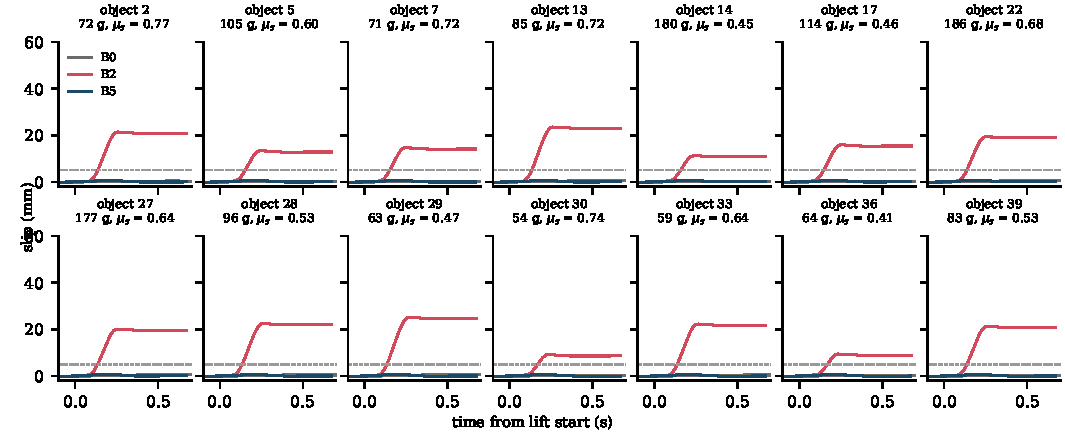
\includegraphics[width=\textwidth]{fig_gallery.pdf}
\caption{\textbf{Every failure of the worst unshielded seed} (B2 seed 2, $r=1.2$, 14 of 40 test objects): slip against time
for the model controller (B0), the unshielded residual (B2) and the shield-trained residual (B5, seed 2) on the same object
and episode seed. All 14 failures share the mechanism of Fig.~\ref{fig:anatomy}; final slips range from 9 to 25\,mm.}\label{fig:gallery}
\end{figure}

\begin{table*}[p]\centering\footnotesize
\caption{\textbf{Per-object test results.} $m$ and $\mu_s$ are the object's mass and static friction; $F_{\rm stuck}/F_b$ is the probed
breakaway grip relative to the true quasi-static breakaway grip $F_b=mg/(2\mu_s)$ (it is $\ge1$ by construction and at most
$1/0.9$ up to sensing noise); probes and probe time are from the B0 episode at $r=1$. Grip columns are $F/mg$ (mean over $r$ and seeds).
B2 failures count lifts with slip $>5$\,mm over 5 seeds $\times$ 4 values of $r$.}\label{tab:perobj}
\setlength{\tabcolsep}{5pt}
\begin{tabular}{@{}rrrrrrrrr@{}}\toprule
Obj & $m$ (g) & $\mu_s$ & $F_{\rm stuck}/F_b$ & probes & probe time (s) & B0 grip & B5 grip & B2 failures\\\midrule
0 & 69 & 0.60 & 1.075 & 7 & 3.9 & 0.95 & 1.28 & 0/20 \\
1 & 140 & 0.41 & 1.051 & 4 & 2.7 & 1.35 & 1.82 & 0/20 \\
2 & 72 & 0.77 & 0.986 & 11 & 5.5 & 0.68 & 0.92 & 11/20 \\
3 & 61 & 0.45 & 1.075 & 5 & 3.1 & 1.26 & 1.69 & 0/20 \\
4 & 192 & 0.65 & 1.054 & 8 & 4.3 & 0.86 & 1.16 & 0/20 \\
5 & 105 & 0.60 & 1.012 & 8 & 4.3 & 0.89 & 1.20 & 3/20 \\
6 & 149 & 0.51 & 1.077 & 7 & 3.9 & 1.12 & 1.51 & 0/20 \\
7 & 71 & 0.72 & 1.001 & 11 & 5.5 & 0.74 & 1.00 & 5/20 \\
8 & 151 & 0.60 & 1.083 & 8 & 4.3 & 0.95 & 1.28 & 0/20 \\
9 & 173 & 0.62 & 1.041 & 8 & 4.3 & 0.89 & 1.20 & 0/20 \\
10 & 197 & 0.48 & 1.029 & 6 & 3.5 & 1.13 & 1.53 & 3/20 \\
11 & 133 & 0.59 & 1.060 & 8 & 4.3 & 0.95 & 1.28 & 0/20 \\
12 & 103 & 0.64 & 1.091 & 9 & 4.7 & 0.91 & 1.23 & 0/20 \\
13 & 85 & 0.72 & 0.983 & 11 & 5.5 & 0.72 & 0.98 & 12/20 \\
14 & 180 & 0.45 & 1.012 & 6 & 3.5 & 1.19 & 1.60 & 6/20 \\
15 & 120 & 0.51 & 1.074 & 6 & 3.5 & 1.11 & 1.50 & 0/20 \\
16 & 62 & 0.76 & 1.028 & 11 & 5.5 & 0.72 & 0.97 & 0/20 \\
17 & 114 & 0.46 & 1.012 & 5 & 3.1 & 1.17 & 1.57 & 3/20 \\
18 & 151 & 0.48 & 1.025 & 6 & 3.5 & 1.13 & 1.52 & 0/20 \\
19 & 185 & 0.49 & 1.025 & 7 & 3.9 & 1.11 & 1.51 & 3/20 \\
20 & 55 & 0.48 & 1.059 & 6 & 3.5 & 1.17 & 1.57 & 0/20 \\
21 & 102 & 0.59 & 1.037 & 8 & 4.3 & 0.93 & 1.26 & 0/20 \\
22 & 186 & 0.68 & 0.990 & 10 & 5.1 & 0.77 & 1.04 & 11/20 \\
23 & 101 & 0.41 & 1.072 & 5 & 3.1 & 1.40 & 1.88 & 0/20 \\
24 & 74 & 0.80 & 1.081 & 11 & 5.5 & 0.72 & 0.97 & 0/20 \\
25 & 119 & 0.68 & 1.043 & 10 & 5.1 & 0.82 & 1.10 & 0/20 \\
26 & 58 & 0.41 & 1.036 & 5 & 3.1 & 1.33 & 1.78 & 0/20 \\
27 & 177 & 0.64 & 0.991 & 9 & 4.7 & 0.83 & 1.12 & 10/20 \\
28 & 96 & 0.53 & 0.990 & 8 & 4.3 & 1.00 & 1.34 & 7/20 \\
29 & 63 & 0.47 & 0.986 & 6 & 3.5 & 1.11 & 1.50 & 6/20 \\
30 & 54 & 0.74 & 1.011 & 10 & 5.1 & 0.73 & 0.98 & 2/20 \\
31 & 120 & 0.45 & 1.066 & 5 & 3.1 & 1.25 & 1.68 & 0/20 \\
32 & 161 & 0.48 & 1.086 & 6 & 3.5 & 1.20 & 1.62 & 0/20 \\
33 & 59 & 0.64 & 0.985 & 9 & 4.7 & 0.82 & 1.10 & 3/20 \\
34 & 184 & 0.41 & 1.087 & 4 & 2.7 & 1.40 & 1.89 & 0/20 \\
35 & 171 & 0.48 & 1.057 & 6 & 3.5 & 1.18 & 1.59 & 0/20 \\
36 & 64 & 0.41 & 1.019 & 5 & 3.1 & 1.33 & 1.78 & 2/20 \\
37 & 94 & 0.69 & 1.076 & 10 & 5.1 & 0.82 & 1.11 & 0/20 \\
38 & 124 & 0.74 & 1.043 & 11 & 5.5 & 0.74 & 1.01 & 0/20 \\
39 & 83 & 0.53 & 0.996 & 7 & 3.9 & 1.00 & 1.35 & 5/20 \\
\bottomrule\end{tabular}\end{table*}

\clearpage
\section{Extended Study Details}\label{app:ext} (pending)


\clearpage
\section{Protocol, Deviations and Reproducibility}\label{app:protocol}
\textbf{Timeline.} The repository history records the order of work: (1) rig, validation and the frozen protocol;
(2) training, test-set evaluation and the analysis code, committed before the confirmation run; (3) the confirmation run,
deviations D1--D3, the exploratory slip-allowance analysis and the first paper draft; (4) Addendum~A, frozen before any of
the extended study was run; (5) the extended study and this paper.

\begin{codebox}{Pre-registered questions and outcomes (excerpt of \texttt{PROTOCOL.md}, frozen before training)}
\small
\textbf{Q1 (speed and grip).} Does a residual lift faster than the model, and how much of that survives the shield?
Outcomes: lift time $T$, relative grip $F/mg$, success. Test B2, B4g, B5 vs B0 per $r$.\\[2pt]
\textbf{Q2 (safety vs r).} Failure rate (drop or slip $>5$\,mm) per method and $r$; is the unshielded residual's failure rate
higher at larger $r$?\\[2pt]
\textbf{Q3 (which axis).} Grip projection (B4g) vs time projection (B4t) on the same commands: $T$, $F/mg$, success,
fraction projected and declined.\\[2pt]
\textbf{Q4 (certificate).} For every shielded episode: fraction with slip $>$ bound, max exceedance, and number with slip
$>S_{\rm tol}$ among certified lifts, at $r\le r_{\max}$ and at $r>r_{\max}$; effect of $r_{\max}=1.0/1.2/1.4$.\\[2pt]
\textbf{Statistics.} Learned methods summarised per object as the mean over 5 seeds; paired Wilcoxon signed-rank tests vs B0
over the 40 objects for $T$ and $F/mg$ at each $r$; Holm correction within each question family; failure rates with Wilson
95\% intervals; exact McNemar tests on per-object any-failure; hierarchical bootstrap 95\% CIs (seeds, then objects; 10{,}000
draws). Only measured results are reported.
\end{codebox}

\textbf{Deviations.} All are dated in the repository.
\begin{itemize}[leftmargin=1.5em]
\item \textbf{D1.} The pre-registered exceedance metric (slip $>$ bound) counts elastic creep: every certified lift had a bound
of exactly zero and 0.05--0.49\,mm of creep. We report it as registered and add the size of the excess and the count of
lifts over the tolerance.
\item \textbf{D2.} The confirmation set draws $r$ per object from $U[1.0,1.3]$, so per-$r$ tests do not apply; it is analysed
pooled over objects with the same tests, plus failures by $r$ band.
\item \textbf{D3.} The slip-allowance analysis (Fig.~\ref{fig:cliffapp}, Table~\ref{tab:allow}) was not pre-registered.
\item \textbf{Addendum A.} The extended study (Section~\ref{sec:extended}, Appendix~\ref{app:ext}) was designed after the
confirmatory results and frozen before it was run. Before running it we refactored module constants used as default
arguments so they are read at call time; re-running 40 randomly chosen test episodes reproduced the committed results
exactly.
\end{itemize}

\textbf{Software and compute.} Python 3.13, MuJoCo 3.15.0, NumPy 2.5, SciPy 1.18, pandas 3.0, statsmodels 0.15,
Matplotlib 3.11. All experiments ran on two cores of a cloud CPU (Intel Xeon, 2.1\,GHz); no GPU was used.
Table~\ref{tab:compute} lists the episodes and wall-clock time.

\begin{table}[!htbp]\centering\small
\caption{\textbf{Compute.} Episodes simulated per experiment and single-core CPU hours at the measured 0.075\,s per episode
(each episode simulates about 6\,s of contact-rich dynamics at 1\,ms). Everything ran on two CPU cores; no GPU.}\label{tab:compute}
\begin{tabular}{@{}lrr@{}}\toprule
Experiment & episodes & CPU hours\\\midrule
Rig validation (V1--V4) & -- & $<0.1$\\
Main training: B2{,} B5 $\times$ 5 seeds & 15{,}600 & 0.3\\
Test set & 5{,}440 & 0.1\\
Confirmation set & 680 & 0.0\\
Training rows T1--T3 (30 runs) & 46{,}800 & 1.0\\
Training row T4 (10 runs{,} 40 iterations) & 31{,}200 & 0.7\\
Controlled rows E1--E9{,} S1--S6 & 52{,}800 & 1.1\\
Controlled rows T1--T4 & 14{,}080 & 0.3\\
Diagnostic rows E7L{,} E9L{,} R0L & 10{,}560 & 0.2\\
Safety map & 10{,}080 & 0.2\\
Bound tightness & 2{,}160 & 0.0\\
\midrule Total & 189{,}400 & 3.9\\
\bottomrule\end{tabular}\end{table}

\begin{codebox}{Reproduce every number}
\small\ttfamily
python validate.py\hfill\# rig validation (Table~\ref{tab:val})\\
./train\_all.sh\hfill\# B2, B5: 5 seeds each\\
python evaluate.py test \&\& python analyze.py test\\
python evaluate.py confirm \&\& python analyze\_confirm.py\\
python explore\_allowance.py\hfill\# D3\\
./train\_extra.sh \&\& python controlled.py ALL\_ENV \&\& python controlled.py ALL\_TRAIN\\
python extended.py tightness \&\& python extended.py safetymap \&\& python extended.py traces\\
python controlled\_analysis.py \&\& python figs\_ext.py ... \&\& python make\_tables.py ...
\end{codebox}
